\begin{slikaDesno}{fig/delay.pdf}
\PID На слици је приказан континуалан систем у 
коме је употребљен идеални појачавач
појачања $A \in \mathbb R$ и 
идеални блок за кашњење
кашњења $\uptau > 0$. Посматра се систем 
чији је 
једини улаз 
сигнал $x = x(t)$ а једини излаз
сигнал $y = y(t)$. 
\end{slikaDesno}


\begin{enumerate}[label=(\alph*)]
    \item Одредити израз за импулсни 
    одзив посматраног система, $h(t)$, 
    и скицирати 
    његов временски дијаграм у интервалу 
    $0 \leq t \leq 5\uptau$. 
    
    \item Полазећи од резултата 
    претходне тачке, испитати BIBO
    стабилност посматраног система у
    зависности од параметара $A$ и 
    $\uptau$. 
    
    \item За вредност параметра $A = 1$, 
    скицирати временски 
    дијаграм одзива датог система на побуду
    $x(t) = \sin(\upomega_0 t)\,\uu(t)$, где је 
    $\upomega_0 = \dfrac{2\uppi}{\uptau}$.     
\end{enumerate} 

\textsc{\myul{Решење:}} 
(а) Означимо оператор кашњења за време $\uptau$ са $\mathrm T_{\uptau}$, односно 
$\mathrm T_{\uptau} x(t) = x(t - \uptau)$. Веза између улазног и излазног
сигнала се може онда записати као $y = A(x + \mathrm T_{\uptau} y)$, одакле се сређивањем добија 
$
    y = \dfrac{A}{1 - A\mathrm T_{\uptau}}  x
$, одакле је оператор система непосредно $\mathrm L = \dfrac{A}{1 - A\mathrm T_{\uptau}}$. 

\textbf{I начин}
Добијени оператор се може итеративно развити у ред по оператору $\mathrm T_{\uptau}$, поступком:
\begin{align}
    \textrm L =& \dfrac{A}{1 - A\mathrm T_{\uptau}} = 
                \dfrac{A \overbrace{- A^2 \mathrm T_{\uptau} + A^2 \mathrm T_{\uptau}}^{+0} }{1 - A\mathrm T_{\uptau}} 
              = A + A\mathrm T_{\uptau} \overbrace{ \dfrac{A}{1 - A\mathrm T_{\uptau}} }^{\mathrm L}  \ldots & \\
              =& A + A^2 T_{\uptau}^2 + A^3 T_{\uptau}^2 + \cdots & 
              = \sum_{k = 1}^{\infty} A^{k} T_{\uptau}^{k-1} \label{\ID.eq1}
\end{align}

\textbf{II начин} по аналогији са изразом за суму геометријског реда,
\begin{equation}
    1 + q + q^2 + q^3 + \cdots = \sum_{k=0}^{\infty} q^k = \dfrac{1}{1 - q},
\end{equation}
без упуштања у питања конвергенције, може се приметити да се добијени оператор може изразити као:
\begin{equation}
    \mathrm L = A\cdot \dfrac{1}{1 - \underbrace{A\mathrm T_{\uptau}}_{q} } =  
               A(1 + A\mathrm T_{\uptau} + A^2\mathrm T_{\uptau}^2 + \cdots) = \sum_{k = 1}^{\infty} A^{k} T_{\uptau}^{k-1} \label{\ID.eq2}
\end{equation}

Оба предложена начина, дати изразима \eqref{\ID.eq1} и \eqref{\ID.eq2} дају исти резултат, па се импулсни одзив на основу тога може добити непосредно директном 
применом оператора као 
\begin{equation}
    h(t) = \mathrm L \updelta(t) = \sum_{k = 1}^{\infty} A^{k} T_{\uptau}^{k-1} \updelta(t) = 
    \sum_{k = 1}^{\infty} A^{k} \updelta(t - (k-1)\uptau),
\end{equation}
којом приликом је искоришћено да је $\mathrm T^k_{\uptau} = \mathrm T_{k\uptau}$, што је тачно у конкретном случају система за кашњење.
Импулсни одзив стога представља поворку Диракових импулса на положајима $(k-1)\uptau$, сваки мере $A^k$, за $k \in \mathbb N$. 
У зависности од тога да ли је параметар $A > 0$ 
већи, мањи, или једнак 1, разликују се три случаја за скицирање графика. 

\begin{figure}[ht!]
    \hspace*{0pt}\hfill
    \begin{subfigure}[c]{0.33\textwidth}
        \centering
        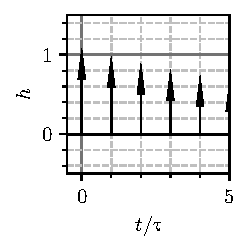
\includegraphics[scale=1]{fig/delay_s1.pdf}
        \caption{$A < 1$}
    \end{subfigure}
    \hspace*{0pt}\hfill
    \begin{subfigure}[c]{0.3\textwidth}
        \centering
        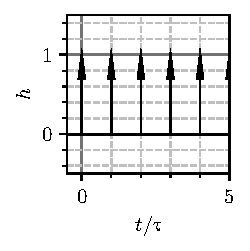
\includegraphics[scale=1]{fig/delay_s2.pdf}
        \caption{$A = 1$}
    \end{subfigure}
    \hfill
    \hspace*{0pt}
    \hspace*{0pt}\hfill
    \begin{subfigure}[c]{0.3\textwidth}
        \centering
        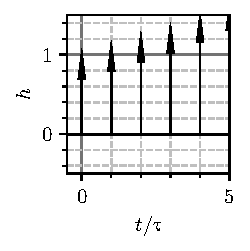
\includegraphics[scale=1]{fig/delay_s3.pdf}
        \caption{$A > 1$}
    \end{subfigure}
    \caption{}
\end{figure}
У случају када је $A < 0$ такође раздвајамо ова три случаја, али онда су импулсни на непарним местима усмерени наниже.

(б) Стабилност датог система може се испитати на начин описан у задатку \ref{z:h_stab}, испитивањем конвергенције  
интеграла апсолутне вредности импулсног одзива, односно,
\begin{equation}
    \int_{-\infty}^{\infty} |h(t)| \, \de t
    = 
    \int_{-\infty}^{\infty} \left\lvert 
    \sum_{k = 1}^{\infty} A^{k} \updelta(t - (k-1)\uptau)
    \right\rvert \, \de t 
    = 
     \sum_{k = 1}^{\infty} |A|^{k} \cancelto{1}{\int_{-\infty}^{\infty} \updelta(t - (k-1)\uptau) t} \, \de t
\end{equation}
Систем је BIBO стабилан дакле у случају да је израз $\sum_{k = 1}^{\infty} |A|^{k}$ конвергентан, што је 
сума геометријског реда, па је услов конвергеције да је $|A| < 1$. Закључујемо, систем је стабилан у BIBO смислу ако је $|A| < 1$,
а нестабилан уколико је $|A| \geq 1$.   

(в) 
У случају када је $A = 1$, оператор таквог система има облик 
$\textrm{L} = \sum_{k = 0}^{\infty} T_{\uptau}^{k}$, па се одзив на побуду $x(t) = \sin(2\uppi t/\uptau)\,\uu(t)$ може 
добити као:
\begin{align}
    y(t) =& \textrm{L} x(t) =  \sum_{k = 0}^{\infty} T_{\uptau}^{k} \sin(2\uppi t/\uptau)\,\uu(t) 
         =  \sum_{k = 0}^{\infty} \sin(2\uppi (t - k\uptau) /\uptau)\,\uu(t - k\uptau) 
         \\
        =& \sum_{k = 0}^{\infty} \underbrace{ \sin(2\uppi t/\uptau - 2\uppi k) }_{\text{Периодичност $\sin$}} \, \uu(t - k\uptau) 
        = \sin(2\uppi t/\uptau) \sum_{k = 0}^{\infty} \uu(t - k\uptau).
    \end{align}
Добијени члан који представља амплитду синусоиде, периоде $\uptau$, мења се степенасто у тренуцима $k\uptau$, тако да се график одзива може скицирати
као што је приказано на слици \ref{fig:\ID.2}. На слици је сивом бојом приказан сигнал 
$\sum_{k = 0}^{\infty} \uu(t - k\uptau)$ који представља степенасто мењање амплитуде синусоиде.


\begin{figure}[ht!]
    \centering
    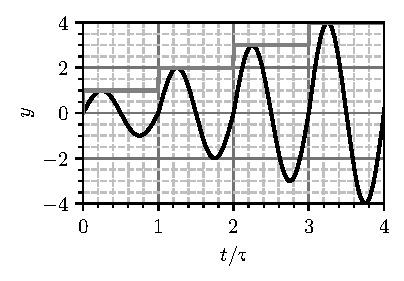
\includegraphics[scale=1]{fig/delay_resp.pdf}
    \caption{}
    \label{fig:\ID.2}
\end{figure}


    \filbreak


